\documentclass[11pt, a4paper]{article}

\usepackage{graphicx}
\usepackage[a4paper,top=3cm,bottom=2cm,left=2cm,right=2cm,marginparwidth=1.75cm]{geometry}
\usepackage[english]{babel}
\usepackage[utf8x]{inputenc}
\usepackage{subfig}
\usepackage{float}
\usepackage{amsmath}
\usepackage{amssymb}
\usepackage{mhchem}
\usepackage{hyperref}
\usepackage{tikz}
\usepackage{cancel}
\usepackage{bm}

\graphicspath{ {./images} }
\newcommand*{\qed}{\hfill\ensuremath{\quad\square}}%
\newcommand*{\rad}{\ensuremath{\,\text{rad}}}
\newcommand*{\R}{\ensuremath{\mathbb{R}}}
\newcommand*{\C}{\ensuremath{\mathbb{C}}}
\renewcommand*{\Re}{\operatorname{Re}}
\renewcommand*{\Im}{\operatorname{Im}}
\renewcommand*{\epsilon}{\varepsilon}
\renewcommand*{\phi}{\varphi}
\renewcommand*{\d}{\text{d}}

\DeclareRobustCommand{\uvec}[1]{{%
  \ifcat\relax\noexpand#1%
    % it should be a Greek letter
    \bm{\hat{#1}}%
  \else
    \ifcsname uvec#1\endcsname
      \csname uvec#1\endcsname
    \else
      \bm{\hat{\mathbf{#1}}}%
     \fi
   \fi
}}

\makeatletter
\renewcommand*\env@matrix[1][*\c@MaxMatrixCols c]{%
  \hskip -\arraycolsep
  \let\@ifnextchar\new@ifnextchar
  \array{#1}}
\makeatother

\newtheorem{theorem}{Theorem}
\numberwithin{equation}{section}
\numberwithin{figure}{section}

%------------------------------------------------
%Templates for images and figures
% \begin{figure}[h]
%   \centering
%   \subfloat[caption 1]{{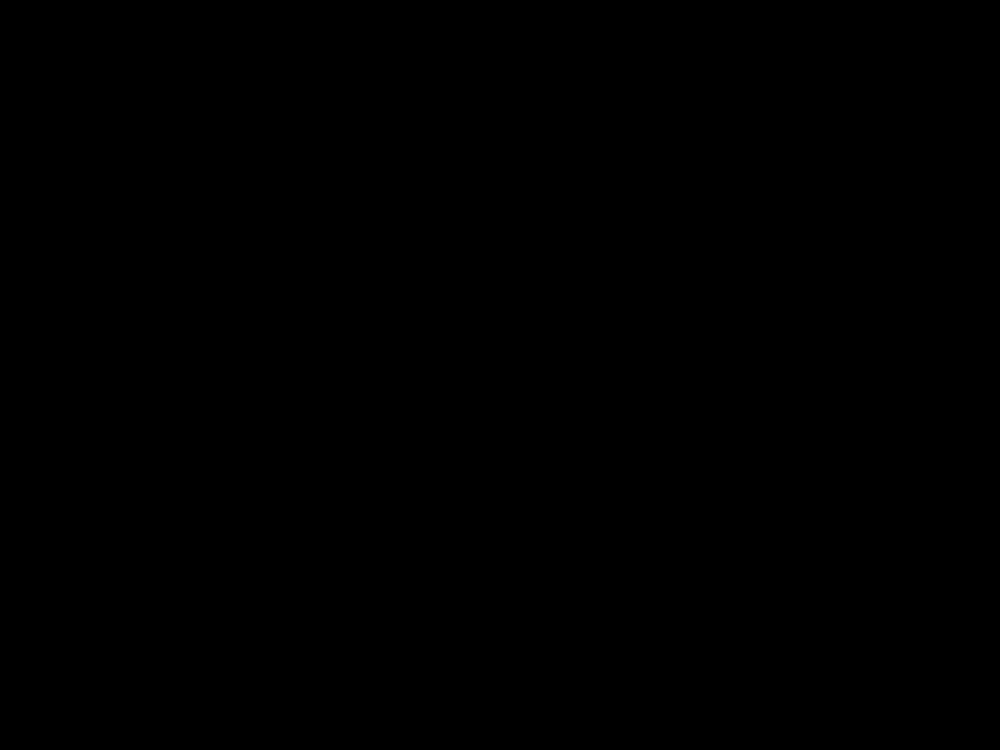
\includegraphics[width=30mm]{images/placeholder.png}}}%
%   \qquad
%   \subfloat[caption 2]{{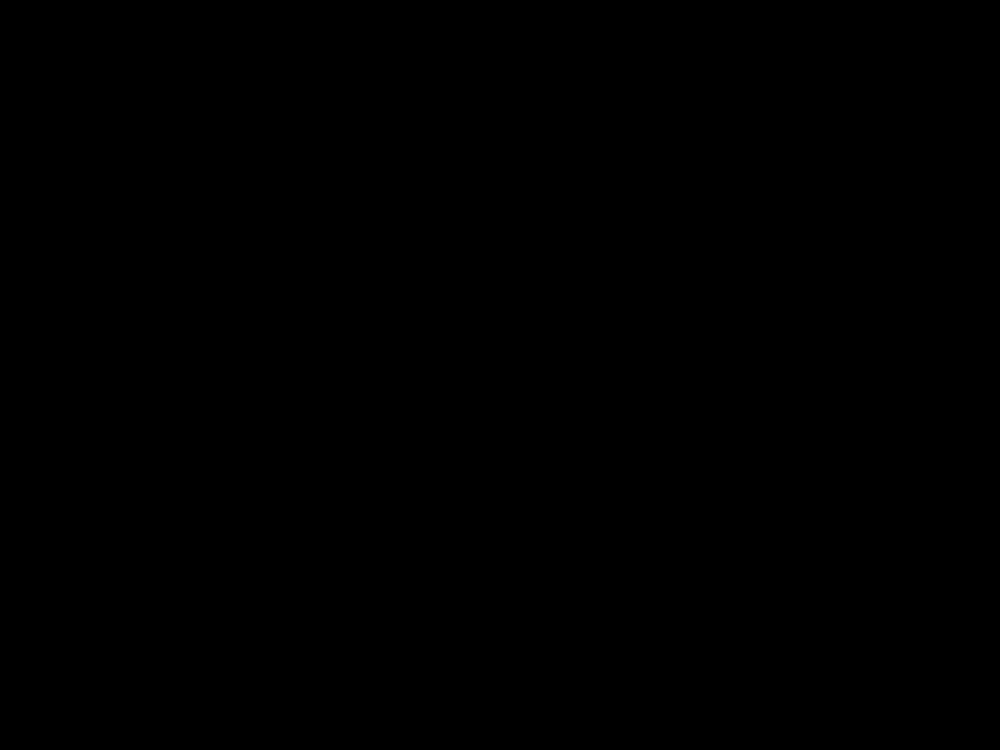
\includegraphics[width=30mm]{images/placeholder.png}}}%
%   \caption{Description}
% \end{figure}

% \begin{figure}[h]
%   \centerline{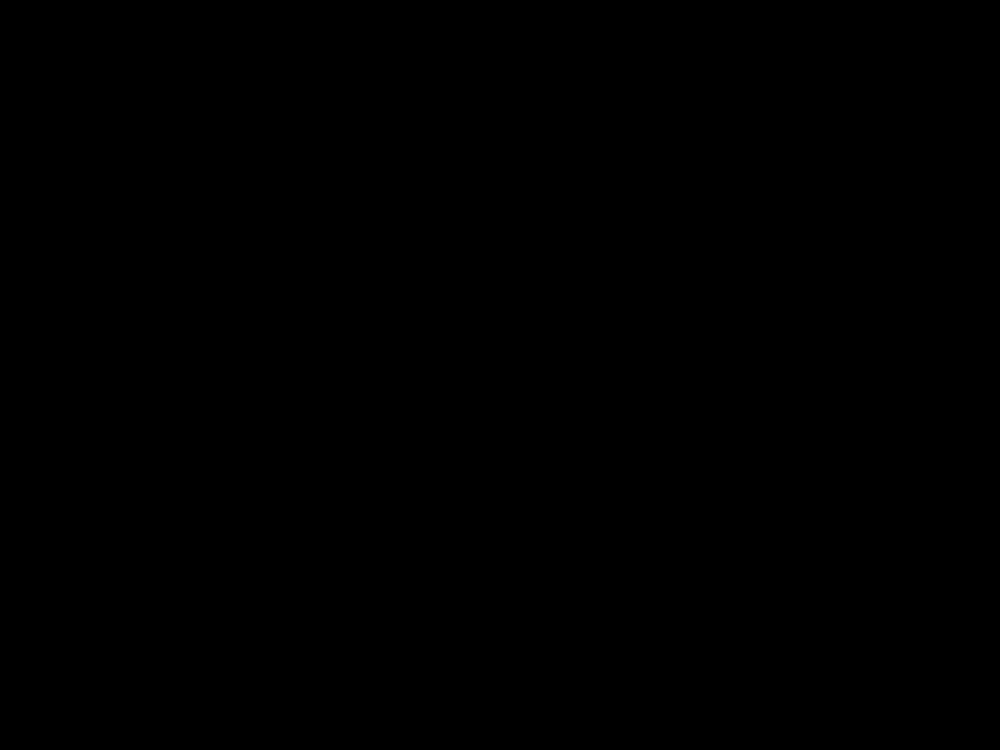
\includegraphics[width=50mm]{images/placeholder.png}}
%   \caption{Description}
% \end{figure}

%Template for a simple table 
%\begin{table}[h]
%   \caption{Description} %title of the table
%   \centering % centering table
%   \begin{tabular}{l rr} % creating three columns
%     \hline\hline %inserting double-line
%     & & \\ [0.5ex] % Insert half line vertical spacing
%     \hline % inserts single-line
%     & & \\ 
%     & & \\
%     & & \\
%     & & \\
%   \hline % inserts single-line
%   \end{tabular}
%   \label{tab:hresult}
% \end{table}
%-----------------------------------------------

\begin{document}
\setcounter{section}{4}
\section{Virtual Work}

\subsection{The principle of virtual work}
Virtual work forms the basis for analytical as well as discrete solution. It is used for finding equillibrium equations in an easier way then the regular solving of $\Sigma F=0$.\\
Conceptually it uses a virtual (imaginary) infinitesimally small displacement $\delta u$ that doesn't disrupt the continuity. The global equillibrium condition for virtual work is:
\begin{equation}
  \delta W_u = 0\; \forall \; \delta\vec{u} \quad \text{while } \delta\epsilon=0
\end{equation}
This means the material will not be deformed. The external virtual work can be expressed as:
\begin{equation}
  \delta W_u = \int_V \left( \rho \vec{f} \cdot \delta\vec{u}\right)\d V + \int_{A_p} \left( \vec{q} \cdot \delta\vec{u} \right)\d A
\end{equation}
This is nothing but an equation expressing energy balance. The material is not deformed thus it can not store any elastic energy. This means all work put into the material must result in some other displacement to maintain balance. Eventhough it is technically an infinitesimal value we can think of $\delta u$ and $\delta W$ practically as some tiny (imaginary) displacement and some tiny amount of work done.\\
\\
\underline{Virtual work exists on our paper and in our head, but cannot be measured and doesn't actually exist in real life.}\\

\underline{Example:}
\begin{figure}[H]
  \centerline{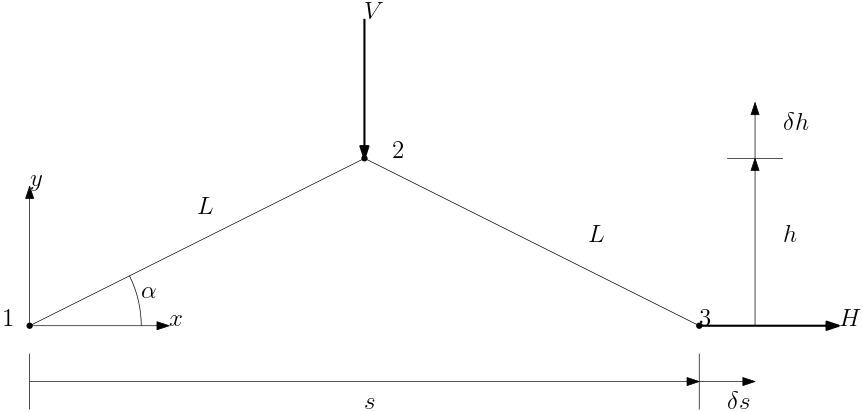
\includegraphics[width=100mm]{images/1.png}}
  \caption{The situation for which we will apply the concept of virtual work to easily figure out the equillibrium equation. Notice that using statics on this problem is kinda awfull since it gives 6 equations and 6 variables for which you'd need to solve.}
\end{figure}
In this case we can use kinematics to find that:
\begin{gather*}
  s = 2L\cos(\alpha)\\
  h = L\sin(\alpha)
\end{gather*}
The equation for virtual work then becomes:
\begin{equation*}
  \delta W_u = H\delta s - V\delta h
\end{equation*}
We could now equate this to $0$ but we would find that $\delta s = \delta h = 0$. The only degree of freedom of the system is the angle $\alpha$. Thus we will express all terms in terms of alpha and solve for that:
\begin{align*}
  \delta s = \frac{\d s}{\d \alpha} \delta\alpha &= \frac{\d(2L\cos(\alpha))}{\d\alpha}\\
  &=-2L\sin(\alpha)\delta\alpha
\end{align*}
\begin{align*}
  \delta h = \frac{\d h}{\d \alpha} \delta\alpha &= \frac{\d(L\sin(\alpha))}{\d\alpha}\\
  &=L\cos(\alpha)\delta\alpha
\end{align*}
This gives the following expression for virtual work:
\begin{equation*}
  \delta W_u = -2HL\sin(\alpha)\delta\alpha - VL\cos(\alpha)\delta\alpha = 0
\end{equation*}
This simplifies to:
\begin{equation*}
  2H\sin(\alpha) + V\cos(\alpha) = 0
\end{equation*}
Which is our equillibrium equation. Since the system has 1 degree of freedom ($\alpha$) we indeed expect to find only 1 equation.


\subsection{Virtual deformations}
We can also allow for virtual deformations to occur. In that case the material will be able to store some elastic energy which changes our equillibrium equations. For the virtual work we get the following for this case:
\begin{equation*}
  \delta W_i = \delta W_u\;\forall\;\delta\vec{u}
\end{equation*}
Which means the internally stored virtual energy in the form of work is the same as the externally applied virtual work. This internal energy takes the form of potential elastic energy which allows us to derrive that:
\begin{equation*}
  \delta W_i = \int_V (\sigma \cdot \delta\epsilon)\d V
\end{equation*}
and
\begin{equation*}
  \delta W_u = \int_V \left( \rho \vec{f} \cdot \delta\vec{u}\right)\d V + \int_{A_p} \left( \vec{q} \cdot \delta\vec{u} \right)\d A
\end{equation*}
\end{document}